\chapter{Umsätze importieren} \label{chap:import}

Über die Ansicht "`Umsätze importieren"' können Kontoauszüge im CSV-Format importiert werden. Aktuell werden ausschließlich Dateien im Exportformat der ING verarbeitet. Die Ansicht ist im Menü unter "`Daten $\rightarrow$ Importieren"' zu finden.

\section{Ablauf: Umsätze importieren}

Eine CSV-Datei kann über den Button "`Datei auswählen"' oder per Drag \& Drop (in jeder Ansicht) importiert werden. Dann werden die gefundenen Umsätze in einer Tabelle angezeigt (s. Abbildung \ref{fig:ImportView}). Sobald eine Importdatei geöffnet wird, findet eine Zuordnung der gefunden Umsätze zu den \textit{regelmäßigen Ausgaben} im System statt. Umsätze, die bereits importiert wurden, werden standardmäßig nicht importiert und mit einer entsprechenden Anmerkung versehen.

Sollte eine Umsatz nicht automatisch einem wiederkehrenden Umsatz zugeordnet werden -- da die Importregeln nicht greifen oder keine konfiguriert wurden --, kann eine manuelle Zuordnung über die Zellen der Spalte "Wiederkehrende Umsätze" vorgenommen werden. Per Doppelklick auf die Zelle öffnet sich ein Dropdown-Menü mit allen wiederkehrenden Umsätzen im System.

\begin{figure}[ht!]
	\centering
	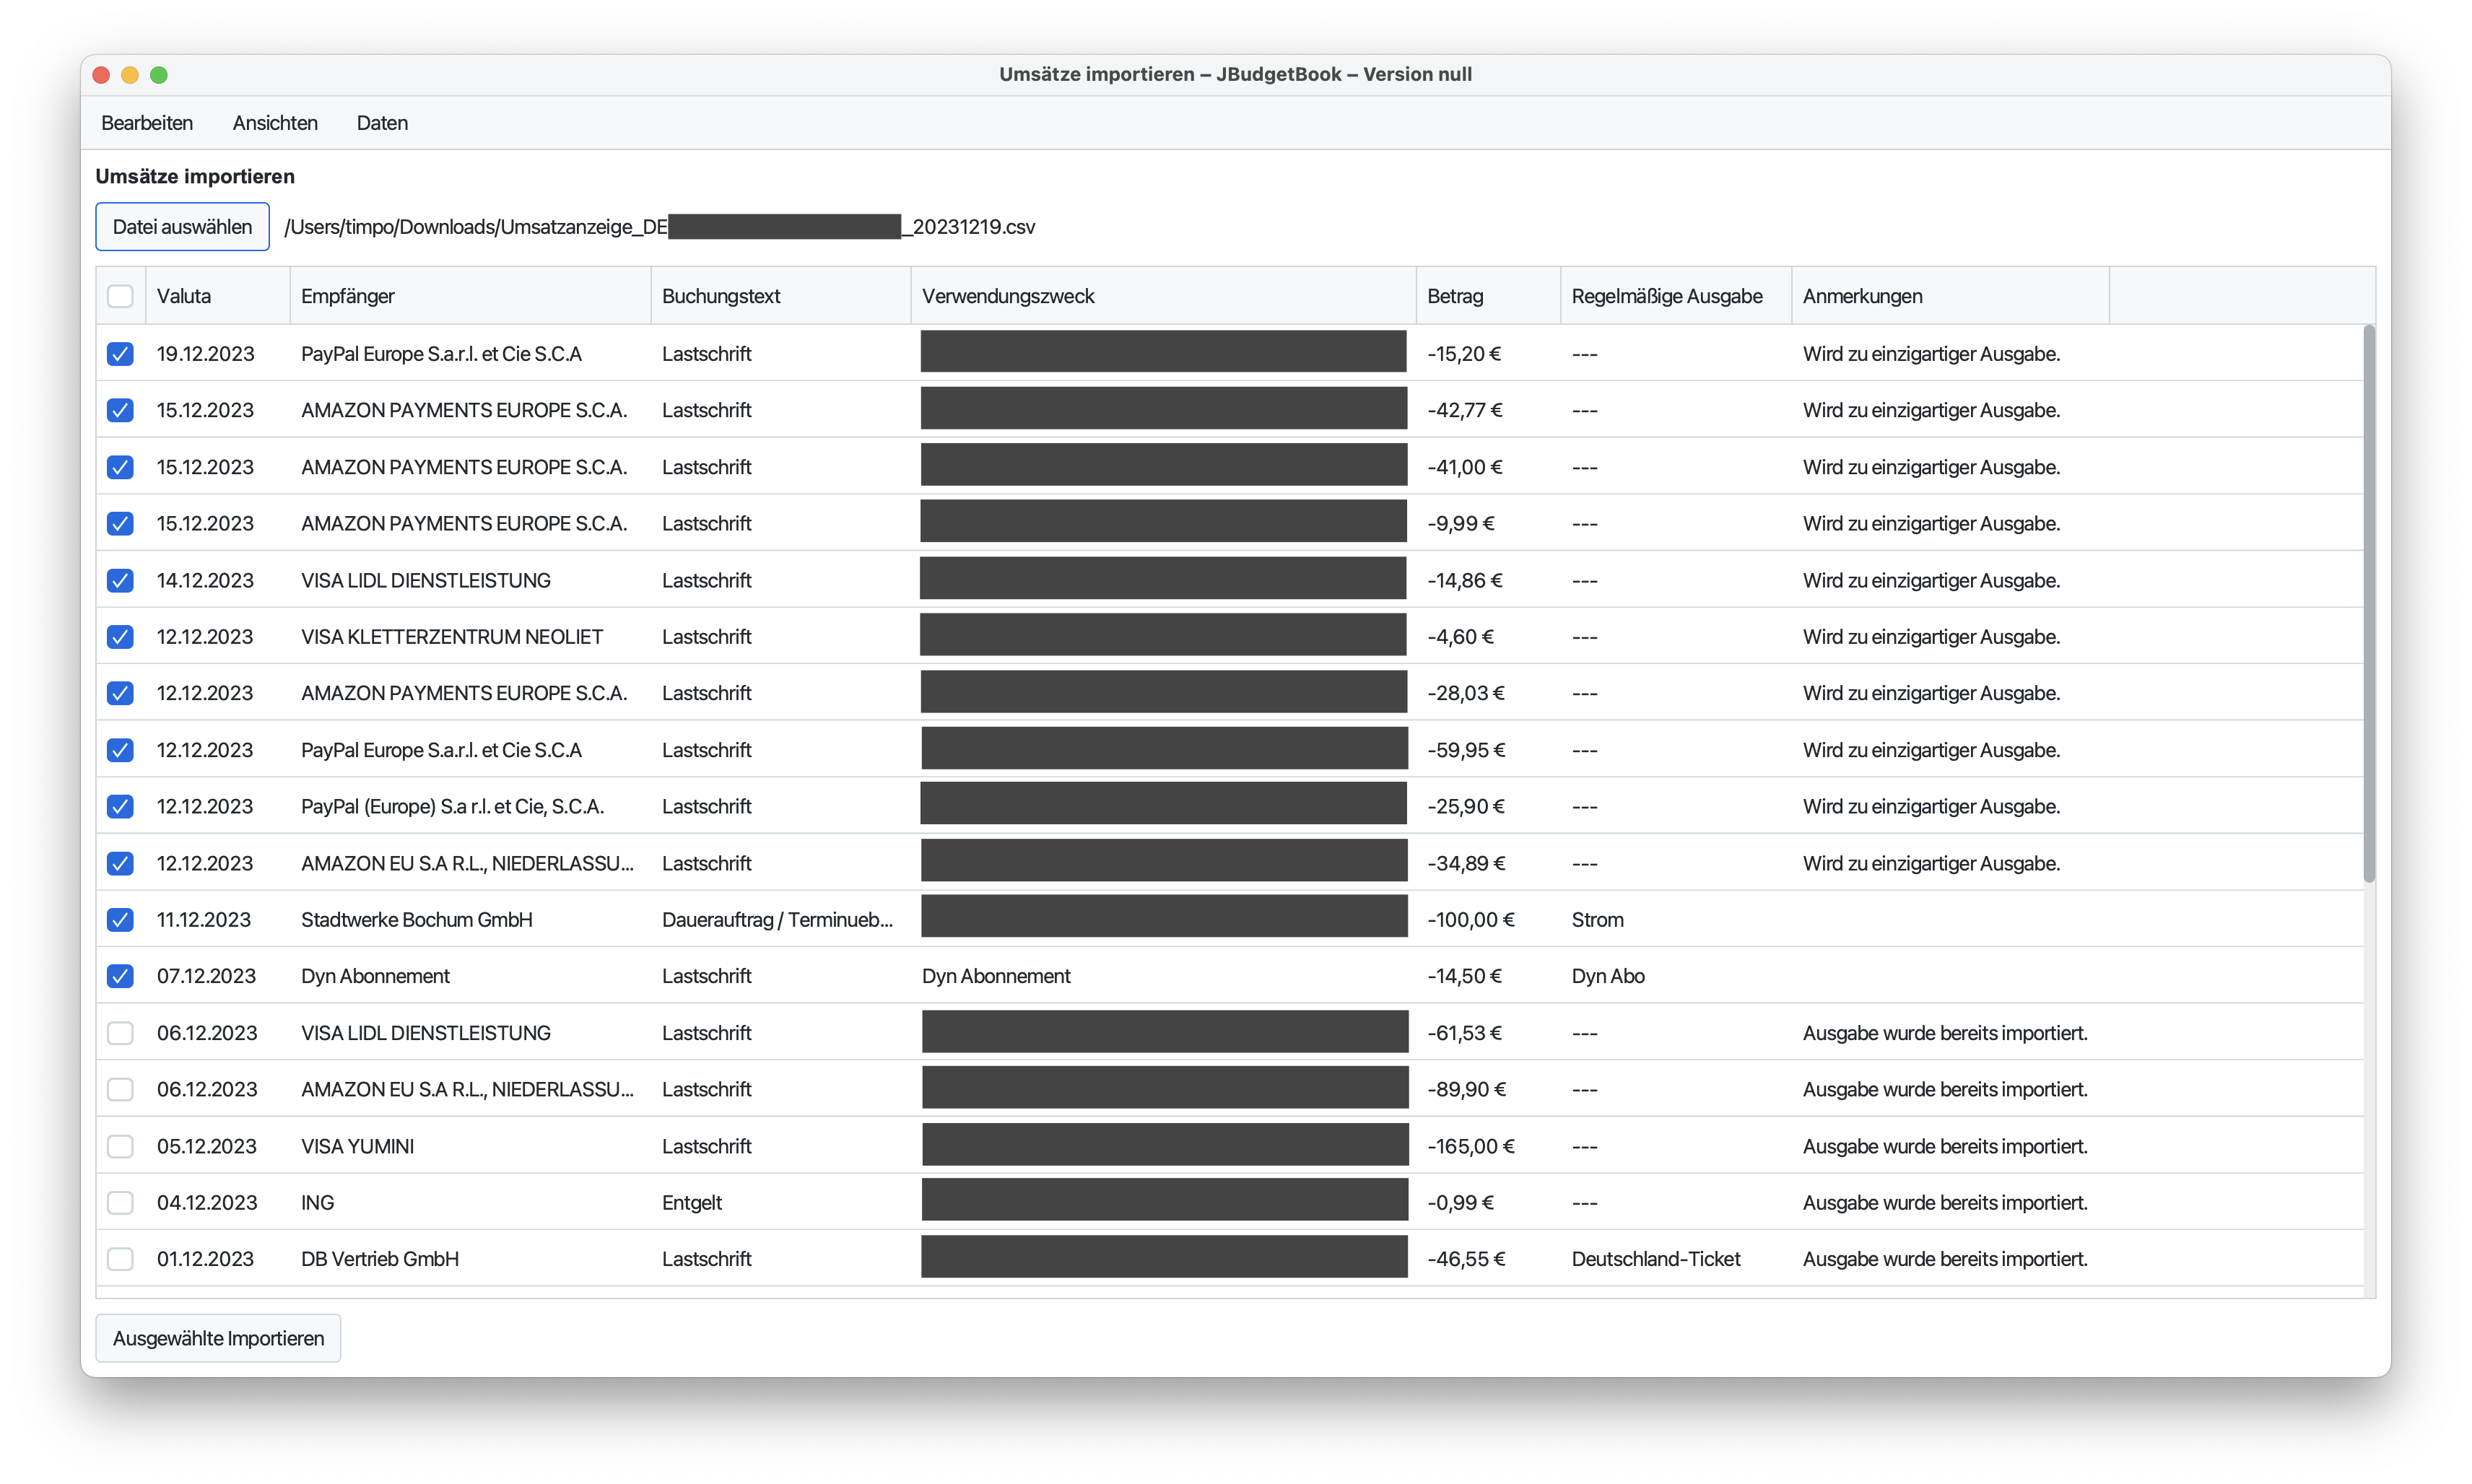
\includegraphics[width=\textwidth]{img/Screenshot-ImportView}
	\vspace{-2em}
	\caption{Ansicht "`Umsätze importieren"'}
	\label{fig:ImportView}
\end{figure}

\section{Importregeln}

Wie reale Umsätze den regelmäßigen Ausgaben zugeordnet werden sollen, kann in der Detailansicht dieser bestimmt werden (s. Abschnitt \ref{sec:fixedExpenses}). Dort kann festgelegt werden, welchen Text der Empfänger oder der Verwendungszweck enthalten muss. Sind Texte in beiden Bedingungen eingetragen, so müssen beide zutreffen (Und-Verknüpfung). 

Unterhalb dieser Konfiguration ist eine Tabelle zu sehen, die die bereits importierten Umsätze zu dieser Ausgabe auflistet. 